\documentclass[preprint,onecolumn,9pt]{sigplanconf} %{onecol}
\usepackage{alltt}
\usepackage{amsmath,amsthm}
\usepackage{amssymb}
\usepackage{stmaryrd}
\usepackage{url}
\usepackage{graphicx}

\newtheorem{theorem}{Theorem}
\newtheorem{lemma}{Lemma}
% \usepackage{xltxtra}
% \setmonofont[Scale=MatchLowercase]{DejaVu Sans Mono}
%
\newcommand{\superscript}[1]{\ensuremath{^{#1}}}
\newcommand{\subscript}[1]{\ensuremath{_{#1}}}
\newcommand{\tuple}[3][\ ]{{\tt #2{#1}}({#3})}

% Values
\newcommand{\clos}[1]{\tuple{clos}{#1}}
\newcommand{\rlos}[1]{\tuple{rlos}{#1}}

% States
\newcommand{\ev}[2][\ ]{\tuple[#1]{ev}{#2}}
\newcommand{\co}[1]{\tuple{co}{#1}}
\newcommand{\ap}[2][\ ]{\tuple[#1]{ap}{#2}}
\newcommand{\ans}[1]{\tuple{ans}{#1}}

% Continuations
\newcommand{\kmt}{\tt mt}
\newcommand{\kar}[2][\ ]{\tuple[#1]{ar}{#2}}
\newcommand{\kfn}[2][\ ]{\tuple[#1]{fn}{#2}}
\newcommand{\kif}[2][\ ]{\tuple[#1]{fi}{#2}}
\newcommand{\kuop}[2][\ ]{\tuple[#1]{oa}{#2}}
\newcommand{\kbopa}[2][\ ]{\tuple[#1]{oa1}{#2}}
\newcommand{\kbopb}[2][\ ]{\tuple[#1]{oa2}{#2}}

% Implementation forms
\newcommand{\generator}{{\tt generator}}
\newcommand{\yield}[1]{{\tt yield} #1}

% Syntax
\newcommand{\syntax}[1]{{\tt #1}}
\newcommand{\sapp}[3][\ ]{\tuple[#1]{app}{#2,#3}}
\newcommand{\slam}[3][\ ]{\tuple[#1]{lam}{#2,#3}}
\newcommand{\srec}[4][\ ]{\tuple[#1]{rec}{#2,#3,#4}}
\newcommand{\svar}[2][\ ]{\tuple[#1]{var}{#2}}
\newcommand{\snum}[2][\ ]{\tuple[#1]{num}{#2}}
\newcommand{\sbln}[2][\ ]{\tuple[#1]{bool}{#2}}
\newcommand{\sif}[4][\ ]{\tuple[#1]{if}{#2,#3,#4}}
\newcommand{\sop}[2][\ ]{\tuple[#1]{op}{#2}}
\newcommand{\sopu}[3][\ ]{\tuple[#1]{op}{#2,#3}}
\newcommand{\sopb}[4][\ ]{\tuple[#1]{op2}{#2,#3,#4}}
\newcommand{\strue}{{\tt tt}}
\newcommand{\sfalse}{{\tt ff}}
\newcommand{\saddone}{{\tt add1}}
\newcommand{\ssubone}{{\tt sub1}}
\newcommand{\szerohuh}{\syntax{zero?}}
\newcommand{\szero}{\syntax{0}}
\newcommand{\slit}[2][\ ]{\tuple[#1]{lit}{#2}}

\newcommand{\sNum}{\syntax{Z}}

% Metavariables
\newcommand{\maddr}{a}
\newcommand{\mvar}{x}
\newcommand{\mvarf}{f}
\newcommand{\mexp}{e}
\newcommand{\mexpi}[1]{e_{#1}}
\newcommand{\mexpf}{f}
\newcommand{\menv}{\rho}
\newcommand{\mkont}{\kappa}
\newcommand{\msto}{\sigma}
\newcommand{\mop}{o}
\newcommand{\mval}{v}
\newcommand{\mnum}{z}
\newcommand{\mbln}{b}
\newcommand{\mvalx}[1]{#1}
\newcommand\machstep{\longmapsto}
\newcommand\multimachstep{\longmapsto\!\!\!\!\!\rightarrow}
\newcommand{\mlit}{l}
\newcommand{\mstate}{\varsigma}
\newcommand{\mcomp}{k}
\newcommand{\mcompi}[1]{\mcomp_{#1}}
\newcommand{\interpdelta}{\Delta}

\newcommand{\compile}[1]{\llbracket#1\rrbracket}

\newcommand{\mlab}{{\ell}}
\newcommand{\mcntr}{{\delta}}
\newcommand{\mtcntr}{{\epsilon}}


\begin{document}

\conferenceinfo{WXYZ '05}{date, City.}
\copyrightyear{2005}
\copyrightdata{[to be supplied]}

% \titlebanner{banner above paper title}        % These are ignored unless
% \preprintfooter{short description of paper}   % 'preprint' option specified.

\title{Optimizing Abstract$^{\text 2}$ Machines}

%% \authorinfo{J. Ian Johnson}
%%            {Northeastern University}
%%            {ianj@ccs.neu.edu}
%% \authorinfo{Matthew Might}
%%            {University of Utah}
%%            {might@cs.utah.edu}
%% \authorinfo{David Van Horn}
%%            {Northeastern University}
%%            {dvanhorn@ccs.neu.edu}
\authorinfo{}{}{}

\maketitle

\begin{abstract}
Abstracting abstract machines has recently been proposed as a
lightweight approach to designing sound and computable program
analyses.  The approach involves deriving abstract interpreters from
existing machine semantics and has been applied to a variety of
languages with features widely considered difficult to analyze.
Although analyzers are straightforward to build under this approach,
the resulting analyzer is prohibitively inefficient.

This article contributes a step by step process for going from a naive
analyzer derived under the abstracting abstract machine approach, to
an efficient program analyzer.
\end{abstract}

%% \category{CR-number}{subcategory}{third-level}

%% \terms
%% term1, term2

%% \keywords
%% keyword1, keyword2

\section{Introduction}

The \emph{abstracting abstract machines}
approach~\cite{dvanhorn:VanHorn2011Abstracting,dvanhorn:VanHorn2012Systematic}
to deriving program analyses provides a straightforward way of
transforming a programming language semantics in the form of an
abstract machine, into a family of abstract interpreters parameterized
over policies for regulating the analytic precision of the control,
environment, store, and base value domains.  By taking a
machine-oriented view of computation, it becomes possible to design,
verify, and implement program analyzers for realistic language
features typically considered difficult to model.  The approach was
originally applied to features such as higher-order functions,
stack-inspection, exceptions, laziness, first-class continuations, and
garbage collection.  It has since been used to verify actor-
\cite{local:DOsualdo:12A} and
thread-based~\cite{dvanhorn:Might2011Family} parallelism and
behavioral contracts~\cite{dvanhorn:TobinHochstadt2012Higherorder}; it
has been used to model Dalvik, Erlang~\cite{local:DOsualdo:12B},
JavaScript~\cite{local:DBLP:journals/corr/abs-1109-4467},
Racket~\cite{dvanhorn:TobinHochstadt2012Higherorder}, and
Coq~\cite{local:harvard}.

The primary strength of the approach is that abstract interpreters can
be easily derived through a small number of steps from existing
machine models. % such as the CESK machine or the Lazy Krivine machine.
Moreover, since the relationships between abstract machines and
higher-level semantic models---such as definitional
interpreters~\cite{dvanhorn:reynolds-hosc98}, structured operational
semantics~\cite{dvanhorn:Plotkin1981Structural}, and reduction
semantics~\cite{dvanhorn:Felleisen2009Semantics}---are well
understood~\cite{dvanhorn:Danvy:DSc}, it is possible to navigate from
these semantic models to sound program analyzers.

%% Using this approach has also lead to new insights in pushdown
%% abstractions of programs capable of precisely modeling the program
%% stack, even in the presence of control effects.




\subsection{Notation and prerequisites}

Prereqs: Semantics Engineering \cite{dvanhorn:Felleisen2009Semantics},
AAM \cite{dvanhorn:VanHorn2011Abstracting}
\cite{dvanhorn:VanHorn2012Systematic}.

Notation: concrete examples of programs under analysis is given in
(monochrome) Scheme notation.  Code is given in (syntax colored)
Racket.

\newpage
\section{Starting point}
\subsection{An abstract$^2$ machine for ISWIM}

ISWIM is a family of programming languages parameterized by a set of
base values and operations.  To make things concrete, we consider a
member of the ISWIM family with integers, booleans, and a few
operations.

\begin{figure}
\[
\begin{array}{l@{\qquad}rcl}
\text{Expressions} & \mathit{e} &=& \svar[^\mlab]\mvar\\
&&|& \slit[^\mlab]\mlit\\
&&|& \slam[^\mlab]\mvar\mexp\\
&&|& \sapp[^\mlab]\mexp\mexp \\
&&|& \sif[^\mlab]\mexp\mexp\mexp \\
\text{Variables}&\mvar &=& \syntax{x}\ |\ \syntax{y}\ |\ \dots\\
\text{Literals}&\mlit &=& \mnum\ |\ \mbln\ |\ \mop\\
\text{Integers}&\mnum &=& \syntax{0}\ |\ \syntax{1}\ |\ \syntax{-1}\ |\ \dots\\
\text{Booleans}&\mbln &=& \strue\ |\ \sfalse\\
\text{Operations}&\mop &=& \syntax{zero?}\ |\ \syntax{add1}\ |\ \syntax{sub1}\ |\ \dots
\end{array}
\]
\caption{Syntax of ISWIM}
\label{fig:syntax}
\end{figure}

Figure~\ref{fig:syntax} defines the (abstract) syntax of ISWIM.
Figure~\ref{fig:aam} defines the semantics of ISWIM as a machine
model.  Evaluation is defined as the set of states reachable by the
reflexive, transitive closure of the machine transition relation.  The
machine is a very slight variation on a standard abstract machine for
ISWIM in ``eval, continue, apply'' form.

Compared with the standard machine semantics, this definition is
different in the following ways:
\begin{itemize}
\item the store maps addresses to \emph{sets} of values,
\item continuations are heap-allocated,
\item there are ``contour values'' (written $\mcntr$) and syntax
  labels ($\mlab$) threaded through the computation, and
\item the machine is implicity parameterized by the functions
  $\mathit{push}$, $\mathit{bind}$, and $\interpdelta$.
\end{itemize}

\begin{figure*}
\begin{align*}
\mathit{eval}(\mexp) &= \{ \mstate\ |\ \ev[^{\mtcntr}]{\mexp,\varnothing,\varnothing,\kmt} \multimachstep \mstate \} \text{ where }
\\[2mm]
%% EVAL
\ev{\svar\mvar,\menv,\msto,\mkont} &\machstep
\co{\mkont,\mval,\msto}
\text{ where }\mval \in \msto(\menv(\mvar))
\\
\ev{\slit\mlit,\menv,\msto,\mkont} &\machstep
\co{\mkont,\mlit,\msto}
\\
\ev{\slam\mvar\mexp,\menv,\msto,\mkont} &\machstep
\co{\mkont,\clos{\mvar,\mexp,\menv},\msto}
\\
\ev[^\mcntr]{\sapp[^\mlab]{\mexpi0}{\mexpi1},\menv,\msto,\mkont} &\machstep
\ev[^\mcntr]{\mexpi{0},\menv,\msto',\kar[_\mlab^\mcntr]{\mexpi{1},\menv,\maddr}}
\text{ where }\maddr,\msto' = \mathit{push}^\mcntr_\mlab(\msto,\mkont)
\\
\ev[^\mcntr]{\sif[^\mlab]{\mexpi0}{\mexpi1}{\mexpi2},\menv,\msto,\mkont} &\machstep
\ev[^\mcntr]{\mexpi0,\menv,\msto',\kif[^\mcntr]{\mexpi1,\mexpi2,\menv,\maddr}}
\text{ where }\maddr,\msto' = \mathit{push}_\mlab^\mcntr(\msto,\mkont)
\\[2mm]
%% CONTINUE
\co{\kmt,\mval,\msto} &\machstep
\ans{\msto,\mval}
\\
\co{\kar[^\mcntr_\mlab]{\mexp,\menv,\maddr},\mval,\msto} & \machstep
\ev[^\mcntr]{\mexp,\menv,\msto,\kfn[^\mcntr_\mlab]{\mval,\maddr}}
\\
\co{\kfn[^\mcntr_\mlab]{{\mvalx{u}},\maddr},\mval,\msto} & \machstep
\ap[^\mcntr_\mlab]{\mval,\mvalx{u},\mkont,\msto}
\text{ where }\mkont \in \msto(\maddr)
\\
\co{\kif[^\mcntr]{\mexpi0,\mexpi1,\menv,\maddr},\strue,\msto} & \machstep
\ev[^\mcntr]{\mexpi0,\menv,\msto,\mkont}
\text{ where }\mkont\in\msto(\maddr)
\\
\co{\kif[^\mcntr]{\mexpi0,\mexpi1,\menv,\maddr},\sfalse,\msto} & \machstep
\ev[^\mcntr]{\mexpi1,\menv,\msto,\mkont}
\text{ where }\mkont\in\msto(\maddr)
\\[2mm]
%% APPLY
\ap[^\mcntr_\mlab]{\clos{\mvar,\mexp,\menv},\mval,\msto,\mkont} & \machstep
\ev[^{\mcntr'}\!]{\mexp,\menv',\msto',\mkont}
\text{ where }\menv',\msto',\mcntr' = \mathit{bind\,}^{ \mcntr}_\mlab(\menv,\msto,\mvar,\mval)
\\
\ap[^\mcntr_\mlab]{\mop,\mval,\msto,\mkont} & \machstep
\co{\mkont,\mval',\msto}
\text{ where } \mval'\in\interpdelta(\mop,\mval)
\end{align*}
\caption{Abstract$^2$ machine for ISWIM}
\label{fig:aam}
\end{figure*}


\paragraph{Concrete interpretation} can be characterized by setting the implicit
parameters of the relation given in Figure~\ref{fig:aam} as follows:
\begin{align*}
\mathit{push}_\mlab^\mcntr(\msto,\mkont) &= \maddr,\msto\sqcup[\maddr\mapsto\{\mkont\}]
\mbox{ where }\maddr \notin\msto
\\
\mathit{bind}(\menv,\msto,\mvar,\mval) &= \menv[\mvar\mapsto\maddr],\msto\sqcup[\maddr\mapsto\{\mval\}]
\mbox{ where }\maddr \notin\msto
\end{align*}
The resulting relation is non-deterministic in its choice of
addresses, however it must always choose a fresh address when
allocating a continuation or variable binding.  If we consider machine
states equivalent up to consistent renaming, this relation defines
a deterministic machine.  (The relation is really a function.)


\paragraph{Abstract interpretation} can be characterized by setting the implicit
parameters just as above, but dropping the $\maddr \not\in \msto$
condition.  This family of interpereters is also non-deterministic in
choices of addresses, but it is free to choose addresses that are
already in use.  Consequently, the machines may be non-deterministic
when mutiple values reside in a store location.

It is important to recognize from this definition that \emph{any}
allocation strategy is an abstract interpretation.  In particular,
concrete intepretation is a kind of abstract interpretation.  So is an
interpretation that allocates a single cell into which all bindings
and continuations are stored.  On the one hand is an abstract
intepretation that is non-computable and gives only the ground truth
of a programs behavior; on the other is an abstract interpretation
that is easy to compute but gives little information.  Useful program
analyses lay somewhere in between and can be characterized by their
choice of address representation and allocation strategy.

%% We now have a framework for describing program analysis for the ISWIM
%% family of languages, whereby approximation of both control and
%% environment structure is regulated by the heap and allocation
%% policies.

Uniform \(k\)-CFA is one such analysis.

\paragraph{Uniform \(k\)-CFA} can be characterized by the following allocation
strategy:

\begin{align*}
\mathit{push}_\mlab^\mcntr(\msto,\mkont) &=
  \mlab\mcntr,\msto\sqcup[\mlab\mcntr\mapsto\{\mkont\}] \\
\mathit{bind}^\mcntr_\mlab(\menv,\msto,\mvar,\mval) &= \menv[\mvar \mapsto \maddr],
                                           \msto\sqcup[\maddr \mapsto
                                             \{ \mval\}],
                                           \mcntr' \\
\mbox{where } \mcntr' &= \lfloor\mlab\mcntr\rfloor_k \\
              \maddr &= x\mcntr' \\
%%              \lfloor \mtcntr \rfloor_k &= \mtcntr \\
              \lfloor \mcntr \rfloor_0 &= \mtcntr \\
              \lfloor \mlab\mcntr \rfloor_{k+1} &= \mlab\lfloor \mcntr\rfloor_k
\end{align*}
%% Redundant
%% \paragraph 0CFA

%% \begin{align*}
%% \mathit{push}(\mlab,\msto,\mkont) &= \mlab,\msto\sqcup[\mlab\mapsto\{\mkont\}]
%% \\
%% \mathit{bind}(\menv,\msto,\mvar,\mval) &= \menv[\mvar\mapsto\mvar],\msto\sqcup[\mvar\mapsto\{\mval\}]
%% \end{align*}


\paragraph{Primitives}



%% \begin{align*}
%% \widehat{\mathit{push}}(\maddr,\msto,\mkont) &= \maddr,\msto\sqcup[\maddr\mapsto\{\mkont\}]
%% % \mbox{ where }\maddr \notin\msto
%% \\
%% \widehat{\mathit{bind}}(\msto,\mvar,\mval) &= \menv[\mvar\mapsto\maddr],\msto\sqcup[\maddr\mapsto\{\mval\}]
%% \end{align*}


\begin{align*}
\mnum+1 &\in \interpdelta(\saddone,\mnum) &
\mnum-1 &\in \interpdelta(\ssubone,\mnum)\\
\strue &\in \interpdelta(\szerohuh,\szero) &
\sfalse &\in \interpdelta(\szerohuh,\mnum)\text{ if }\mnum\neq \szero\\
\end{align*}

\begin{align*}
\sNum &\in \hat\interpdelta(\saddone,\mnum) &
\sNum &\in \hat\interpdelta(\ssubone,\mnum)\\
\strue &\in \hat\interpdelta(\szerohuh,\sNum) &
\sfalse &\in \hat\interpdelta(\szerohuh,\sNum)\\
\strue &\in \hat\interpdelta(\szerohuh,\szero) &
\sfalse &\in \hat\interpdelta(\szerohuh,\mnum)\text{ if }\mnum\neq \szero\\
\end{align*}

HERE: ρ

\begin{figure}
\begin{alltt}
  ;; State \(\to\) Set[State]
  (define (step \(\mstate\))
    (match \(\mstate\)
      [(ev \(\mexp\) \(\rho\) \(\msto\) \(\mkont\))
       (match \(\mexp\)
         [(var\(\superscript\mlab\) \(\mvar\))
          (for/set ((\(\mval\) (lookup \(\rho\) \(\msto\) \(\mvar\))))
            (co \(\msto\) \(\mkont\) \(\mval\)))]
         [(lit\(\superscript\mlab\) \(\mlit\)) (set (co \(\msto\) \(\mkont\) \(\mlit\)))]
         [(lam\(\superscript\mlab\) \(\mvar\) \(\mexp\)) (set (co \(\msto\) \(\mkont\) (clos \(\mvar\) \(\mexp\) \(\rho\))))]
         [(app\(\superscript\mlab\) \(\mexp\subscript0\) \(\mexp\subscript1\))
          (define-values (\(\msto'\) \(\maddr\)) (push \(\mstate\)))
          (set (ev \(\mexp\subscript0\) \(\rho\) \(\msto'\) (ar \(\mexp\subscript1\) \(\rho\) \(\maddr\))))]
         [(ife\(\superscript\mlab\) \(\mexp\subscript0\) \(\mexp\subscript1\) \(\mexp\subscript2\))
          (define-values (\(\msto'\) \(\maddr\)) (push \(\mstate\)))
          (set (ev \(\mexp\subscript0\) \(\rho\) \(\msto'\) (ifk \(\mexp\subscript1\) \(\mexp\subscript2\) \(\rho\) \(\maddr\))))])]
      [(co \(\msto\) \(\mkont\) \(\mval\))
       (match \(\mkont\)
         ['mt (set (ans \(\msto\) \(\mval\)))]
         [(ar\(\superscript\mlab\) \(\mexp\) \(\rho\)) (set (ev \(\mexp\) \(\rho\) \(\msto\) (fn \(\mval\) l)))]
         [(fn\(\superscript\mlab\) \(\mval'\))
          (for/set ((\(\mkont\) (get-cont \(\msto\) l)))
            (ap \(\msto\) \(\mval'\) \(\mval\) \(\mkont\)))]
         [(fi\(\superscript\mlab\) c a \(\rho\))
          (for/set ((k (get-cont \(\msto\) l)))
            (ev (if v c \(\maddr\)) \(\rho\) \(\msto\) \(\mkont\)))])]
      [(ap \(\msto\) fun \(\maddr\) \(\mkont\))
       (match fun
         [(clos l \(\mvar\) \(\mexp\) \(\rho\))
          (define-values (\(\rho'\) \(\msto'\)) (bind \(\mstate\)))
          (set (ev \(\msto'\) \(\mexp\) \(\rho'\) \(\mkont\)))]
         [(op \(\mop\))
          (for*/set ((\(\mkont\) (get-cont \(\msto\) l))
                     (\(\mval\) (\(\interpdelta\) \(\mop\) \(\mval\))))
            (co \(\msto\) \(\mkont\) \(\mval\)))]
         [_ (set)]))]))
\end{alltt}
\caption{Implementation of machine transition relation.}
\end{figure}

\subsection{An example: Analyzing Church number computations}

\newcommand{\church}[1]{\(\ulcorner{\tt #1}\urcorner\)}

%% \begin{alltt}
%% (define \church2 (\(\lambda\) (f) (\(\lambda\) (x) (f (f x)))))

%% (define pred
%%   (\(\lambda\) (n)
%%     (\(\lambda\) (rf)
%%       (\(\lambda\) (rx)
%%         (((n (\(\lambda\) (g) (\(\lambda\) (h) (h (g rf)))))
%%           (\(\lambda\) (i) rx))
%%          (\(\lambda\) (id) id))))))
%% \end{alltt}


%% (define \church0 (\(\lambda\) (f0) (\(\lambda\) (x0) x0)))
%% (define \church1 (\(\lambda\) (f1) (\(\lambda\) (x1) (f1 x1))))
%% (define \church2 (\(\lambda\) (f2) (\(\lambda\) (x2) (f2 (f2 x2)))))
%% (define \church3 (\(\lambda\) (f3) (\(\lambda\) (x3) (f3 (f3 (f3 x3))))))

\begin{figure}
\begin{alltt}
(define ((((plus p1) p2) pf) x)
  ((p1 pf) ((p2 pf) x)))

(define (((mult m1) m2) mf)
  (m2 (m1 mf)))

(define (((pred n) rf) rx)
  (((n (\(\lambda\) (g) (\(\lambda\) (h) (h (g rf)))))
    (\(\lambda\) (ignored) rx))
   (\(\lambda\) (id) id)))

(define (zero? n)
  ((n (\(\lambda\) (zx) #f)) #t))

(define ((church=? e1) e2)
  (if (zero? e1) (zero? e2)
      (if (zero? e2) #f
          ((church=? (pred e1)) (pred e2)))))

;; multiplication distributes over addition
((church=? ((mult \church2) ((plus \church1) \church3)))
 ((plus ((mult \church2) \church1)) ((mult \church2) \church3)))
\end{alltt}
\caption{Church-numeral calculation}
\end{figure}

Where \syntax{church=?} is an equality function for Church numerals
written in terms of recursion and an iterative \syntax{pred} function.
The \syntax{plus} and \syntax{mult} functions are written as usual.

This program reaches $N$ states under concrete interpretation.

\newpage
\subsection{Generic fixpoint calculator}

\begin{alltt}
;; Expr \(\to\) Set[State]
(define (eval e)
  (fix step (set (inj e))))
\end{alltt}

We compute the semantics of a program by iterating the state
transition relation until a fixed point in the reachable states is
reached.

\begin{alltt}
;; \(\forall\) (X) ((X \(\to\) Set[X]) \(\to\) (Set[X] \(\to\) Set[X]))
(define ((appl f) s)
  (for/fold ([i (set)])
    ([x (in-set s)])
    (\(\cup\) i (f x))))

;; Calculate fixpoint of (appl f).
;; \(\forall\) (X) ((X \(\to\) Set[X]) Set[X] \(\to\) Set[X])
(define (fix f s)
  (let loop ((accum (set)) (front s))
    (if (set-empty? front)
        accum
        (let ((new-front ((appl f) front)))
          (loop (\(\cup\) accum front)
                (new-front . \(\setminus\) . accum))))))
\end{alltt}

\subsection{Store widening}

\begin{alltt}
;; \(\widehat{State}\) = (cons (Set Conf) Store)

;; (State \(\to\) Set[State]) \(\to\) \(\widehat{State}\) \(\to\) \(\widehat{State}\)
(define ((wide-step step) state)
  (match state
    [(cons cs \(\msto\))
     (define ss ((appl step)
                 (for/set ([c cs]) (c->s c \(\msto\)))))
     (set (cons (for/set ([s ss]) (s->c s))
                (\(\sqcup\)-stores ss)))]))
\end{alltt}

\subsection{Baseline evaluation}

Wide Store: cpu time: 551571 real time: 571319 gc time: 4003

\section{Precision preserving recipe}

We discuss a variety of techniques for increasing performance by
decreasing the interpretive overhead of abstract interpretation, all
in the purely functional realm. These techniques are the following:
\begin{itemize}
 \item{shrink state space by quotients (lazy non-determinism)}
 \item{shrink state space by removing {\tt ev} states (abstract
   compilation)}
 \item{decrease intermediate data structures by specializing our
fixpoint operator to work with widened machine configurations
(fixpoint specialization)}
 \item{decrease intermediate data structures by operating on store
   changes rather than whole stores (store deltas)}
\end{itemize}
Each technique requires minimal changes to the reduction
relation/fixpoint, and each improves performance by integer factors.

\subsection{Lazy non-determinism}

The first problem that we realized with the AAM approach was that much
of the non-determinism is spurious. For example, in a function
application,
\begin{alltt}
(f x y z w)
\end{alltt}
where all variables have been joined with multiple values, each
variable reference transitions to several new states that comprise the
cartesian product of all the values of {\tt x}, {\tt y}, {\tt z} and
{\tt w}, only to be joined back together in {\tt f}'s bindings. For
this reason, we {\it delay} the non-determinism until it is needed in
{\it strict contexts} (such as the guard for an {\tt if} a called
procedure, or a numerical primitive application).

For this, we introduce a new value for a delayed lookup that acts to
quotient the state space by the values at the delayed address.

\begin{align*}
force(\msto,\clos{\mvar,\mexp,\menv}) &= \{\clos{\mvar,\mexp,\menv}\}\\
force(\msto,\saddr\maddralt) &= \msto(\maddralt)\\
\ev{\svar{\mvar},\menv,\mkont,\msto} &\machstep\;
\co{\mkont,\saddr{\menv(\mvar)},\msto} \\
\co{\kar[^\mcntr_\mlab]{\mexp,\menv,\maddr},v,\msto}
&\machstep\;
\ev[^\mcntr]{\mexp,\menv,\msto,\kfn[^\mcntr_\mlab]{\mval,\maddr}} \\
\mbox{where } &\mval' \in force(\msto,\mval) \\
bind^\mcntr_\mlab(\menv,\msto,\mvar,\mval) &= \menv[\mvar \mapsto
  \maddr], \msto\sqcup[\maddr \mapsto force(\msto, \mval)], \mcntr' \\
\mbox{where } \mcntr' &= \lfloor\mlab\mcntr\rfloor_k \\
              \maddr &= \mvar\mcntr'
\end{align*}

The force for the second rule is necessary to keep the same type for
the \(\kfn{}\) continuation, but we would rather use an address. This
introduces (acceptably) more imprecision, but has the same precision as an ANF
analysis\footnote{Exercise for the reader.}.

Lazy:
   cpu time: 32481 real time: 32881 gc time: 547

\subsection{Abstract compilation}

We can eliminate the {\tt ev} states from the run-time interpretation
of a program by specializing the machine transition relation to the
program being analyzed. This eliminates interpretative overhead by
first compiling the program into ``byte code'' instructions.

The essence of the compilation effect can be seen by consider an example
such as
\[
\sapp{\sapp{\sapp\mvar{\mexp_1}}{\mexp_2}}{\mexp_3}
\]
which makes the following transitions:
\begin{align}
& \ev{\sapp{\sapp{\sapp\mvar{\mexp_1}}{\mexp_2}}{\mexp_3},\menv,\mkont,\msto_0}\\
\machstep\; &
\ev{\sapp{\sapp\mvar{\mexp_1}}{\mexp_2},\menv,\kar{\mexp_3,\menv,\maddr_1},\msto_1}
\\
\machstep\; &
\ev{\sapp\mvar{\mexp_1},\menv,\kar{\mexp_2,\menv,\maddr_2},\msto_2}
\\
\machstep\; &
\ev{\mvar, \menv,\kar{\mexp_1,\menv,\maddr_3},\msto_3} % {\mexp_2}
\\
\machstep\; &
\co{\kar{\mexp_1,\menv},\mval,\msto_4} % {\mexp_1}{\mexp_2}
\mbox{ where } \mval \in \msto(\menv(\maddr))
\end{align}

where $\msto_4 = \msto_0 \sqcup \{ [\maddr_1 \mapsto \{ \mkont \}],
[\maddr_2 \mapsto \kar{\mexp_3,\menv,\maddr_1}]
[\maddr_3 \mapsto \kar{\mexp_2,\menv,\maddr_2}]$.


Notice that the only difference between concrete and abstract interpretation
is which addresses are pushed.

\begin{figure}
\begin{align*}
\compile{\svar\mvar} &= \lambda(\menv,\msto,\mkont) .\co{\mkont,\mval,\msto} \text{ where }\mval\in\msto(\menv(\mvar))
\\
\compile{\slit\mlit} &= \lambda(\menv,\msto,\mkont) .
\co{\mkont,\mlit,\msto}
\\
\compile{\slam\mvar\mexp} &= \lambda(\menv,\msto,\mkont) .
\co{\mkont,\clos{\mvar,\compile\mexp,\menv},\msto}
\\
\compile{\sapp[^\mlab]{\mexpi0}{\mexpi1}} &= \lambda^\mcntr(\menv,\msto,\mkont) .
\compile{\mexpi0}^\mcntr(\menv,\msto',\kar[_\mlab^\mcntr]{\compile{\mexpi1},\menv,\maddr})
\\
&
\text{ where }\maddr,\msto' = \mathit{push}^\mcntr_\mlab(\msto,\mkont)
\\
\compile{\sif[^\mlab]{\mexpi0}{\mexpi1}{\mexpi2}} &= \lambda^\mcntr(\menv,\msto,\mkont) .
\compile{\mexpi0}^\delta(\menv,\msto',\kif[^\mcntr]{\compile{\mexpi1},\compile{\mexpi2},\menv,\maddr})
\\
&\text{ where }\maddr,\msto' = \mathit{push}_\mlab^\mcntr(\msto,\mkont)
\end{align*}
\caption{Compilation}
\end{figure}

\begin{figure}
\begin{align*}
\mathit{eval}(\mexp) &= \{ \mstate\ |\ \compile{\mexp}(\epsilon,\varnothing,\varnothing,\kmt) \multimachstep \mstate \} \text{ where }
\\[2mm]
%% CONTINUE
\co{\kmt,\mval,\msto} &\machstep
\ans{\msto,\mval}
\\
\co{\kar[^\mcntr_\mlab]{\mcomp,\menv,\maddr},\mval,\msto} & \machstep
\mcomp^\mcntr(\menv,\msto,\kfn[^\mcntr_\mlab]{\mval,\maddr})
\\
\co{\kfn[^\mcntr_\mlab]{{\mvalx{u}},\maddr},\mval,\msto} & \machstep
\ap[^\mcntr_\mlab]{\mval,\mvalx{u},\mkont,\msto}
\text{ where }\mkont \in \msto(\maddr)
\\
\co{\kif[^\mcntr]{\mcompi0,\mcompi1,\menv,\maddr},\strue,\msto} & \machstep
\mcompi0^\mcntr(\menv,\msto,\mkont)
\text{ where }\mkont\in\msto(\maddr)
\\
\co{\kif[^\mcntr]{\mcompi0,\mcompi1,\menv,\maddr},\sfalse,\msto} & \machstep
\mcompi1^\mcntr(\menv,\msto,\mkont)
\text{ where }\mkont\in\msto(\maddr)
\\[2mm]
%% APPLY
\ap[^\mcntr_\mlab]{\clos{\mvar,\mcomp,\menv},\mval,\msto,\mkont} & \machstep
\mcomp^{\mcntr'}(\menv',\msto',\mkont) \\
\text{ where }\menv',\msto',\mcntr' &= \mathit{bind\,}^{ \mcntr}_\mlab(\msto,\mvar,\mval)
\\
\ap{\mop,\mval,\msto,\mkont} & \machstep
\co{\mkont,\mval',\msto} \\
\text{ where }\mkont &\in\msto(\maddr)
\text{ and } \mval'\in\interpdelta(\mop,\mval)
\end{align*}
\caption{Abstract$^2$ machine for compiled ISWIM}
\label{fig:caam}
\end{figure}


Compile:
   cpu time: 255397 real time: 261532 gc time: 2947

\noindent
Compile + Lazy:
   cpu time: 31173 real time: 31642 gc time: 739

\newpage
\subsection{Fixed-point specialization}

\begin{alltt}
;; \(\widehat{State} \to \widehat{State}\)
(define (wide-step-specialized state)
  (match state
    [(cons \(\msto\) cs)
     (define-values (cs* \(\msto\)*)
       (for/fold ([cs* \(\varnothing\)] [\(\msto\)* \(\msto\)])
         ([c cs])
         (match (step-compiled^ (cons \(\msto\) c))
           [(cons \(\msto\)** cs**)
            (values (\(\cup\) cs* cs**) (\(\sqcup\)-store \(\msto\)* \(\msto\)**))])))
     (cons \(\msto\)* (\(\cup\) cs cs*))]))
\end{alltt}
%% Should be commutted to beginning

Special + Compile + Lazy:
   cpu time: 14212 real time: 14681 gc time: 823

\subsection{Computing with store changes}

\begin{alltt}
;; \(\widehat{State} \to \widehat{State}\)
(define (wide-step-specialized state)
  (match state
    [(cons \(\msto\) cs)
     (define-values (cs* \(\msdiff\))
       (for/fold ([cs* (set)] [\(\msdiff\)* '()])
         ([c cs])
         (match (step-compiled^ (cons \(\msto\) c))
           [(cons \(\msdiff\)** cs**)
            (values (\(\cup\) cs* cs**) (++ \(\msdiff\)** \(\msdiff\)*))])))
     (cons (update \(\msdiff\) \(\msto\)) (\(\cup\) cs cs*))]))
\end{alltt}

\[
\{ \widehat{v_3}, \widehat{v_5}, \widehat{v_6} \} = 0001011
\]

\[
\sigma = \mbox{\tt \#(0$_0$,\dots,0$_{|P|}$)}
\]

Delta Store + Special + Compile + Lazy:
   cpu time: 668 real time: 686 gc time: 41

\section{Sacrificing precision for performance}

Each step in the fixpointer for the above techniques requires joining
several (possibly large) stores together. Even with immutable hashes
that utilize sharing, this is memory-intensive. Worse, this
contributes an obscene fraction of the runtime. We reuse a technique
created in Shivers' dissertation~\cite{ianjohnson:Shivers:1991:CFA},
timestamp approximation, that removes the need for joining whole
stores by manipulating a global store imperatively. This loses
precision because the starting store for each state in a machine
configuration can change between stepping all states and introduce
more flows than originally possible. The example in figure
\ref{fig:timestamp} illustrates this loss in precision. {\bf TODO:}
EXPLANATION OF LOSS. In many applications, this is acceptable for the
performance improvement.

\begin{figure}
TODO
\caption{Precision lossy program in timestamp approximation}
\label{fig:timestamp}
\end{figure}


% For David to fill in.
\subsection{Imperative global store and worklist}
...
\subsection{Pre-allocated global store}
...

% Ian's sections: generators, implementation and compound data
\section{Implementation}

All the above techniques can be combined into a single implementation
of the small step reduction relation and simple variations of a
general fixpoint combinator. We implementated all of these ideas in an
analysis of core Scheme (call-by-value lambda calculus extended with
variable-arity functions, call/cc, vectors, conses, recursive binding,
various primitives) in just 3000 lines of Racket. Most lines are spent
defining the primitives and expected library functions used in our
benchmarks. Here we describe the unifying vocabulary for writing such
a framework, and some design decisions related to scaling to a
language with compound data.

\subsection{Vocabulary of Parameterized Optimizations}

We combine the interface of generators~\cite{ianjohnson:cluhistory}
with a special lambda form ({\tt $\lambda$\%}) that wraps the meanings
of {\tt ev} states. We also have a special {\tt do} form that performs
behind-the-scenes state passing and iteration much like {\tt do} in
Haskell. In the presence of the different optimization
techniques, {\tt generator}, {\tt yield}, {\tt $\lambda$\%} and {\tt do}
change meaning slightly, but keep the same interface as their names
suggest.

\begin{figure}
\begin{alltt}
\(e-dispatch =\)
(match e
  [(var\(\superscript\mlab\) x)
   (\(\lambda\)\% (\(\msto\) \(\menv\) k)
    (do (\(\msto\)) ((v (delay (lookup-env \(\menv\) x))))
      (yield (co \(\msto\) k v))))]
  [(lit\(\superscript\mlab\) l)
   (\(\lambda\)\% (\(\msto\) \(\menv\) k)
    (do (\(\msto\)) () (yield (co \(\msto\) k n))))]
  [(lam\(\superscript\mlab\) x e)
   (define c (compile e))
   (\(\lambda\)\% (\(\msto\) \(\menv\) k)
    (do (\(\msto\)) () (yield (co \(\msto\) k (clos x c \(\menv\))))))]
  [(app\(\superscript\mlab\) f e)
   (define cf (compile f))
   (define ce (compile e))
   (\(\lambda\)\% (\(\msto\) \(\menv\) k)
    (define-values (\(\msto\)* a) (push state))
    (yield (ev \(\msto\)* cf \(\menv\) (ar c \(\menv\) a))))]
  [(ife\(\superscript\mlab\) e0 e1 e2)
   (define c0 (compile e0))
   (define c1 (compile e1))
   (define c2 (compile e2))
   (\(\lambda\)\% (\(\msto\) \(\menv\) k)
     (do (\(\msto\)) [(\(\msto\)* a) (push state)]
      (yield (ev \(\msto\)* c0 \(\menv\) (ifk c1 c2 \(\menv\) a)))))])

(define (step state)
  (match state
    [(ev \(\msto\) e \(\menv\) k) \(e-dispatch\)] ;; dead if compiled.
    [(co \(\msto\) k v)
     (match k
       ['mt (generator (do (\(\msto\)) ([v <- (force \(\msto\) v)])
        (yield (ans \(\msto\) v))))]
       [(ar\(\superscript\mlab\) e \(\menv\))
        (generator (do (\(\msto\)) ()
          (yield (ev \(\msto\) e \(\menv\) (fn v l)))))
       [(fn\(\superscript\mlab\) f)
        (generator (do (\(\msto\)) ([k <- (get-cont \(\msto\) l)])
         (yield (ap \(\msto\) f v k))))]
       [(fi\(\superscript\mlab\) c a \(\menv\))
        (generator
         (do (\(\msto\)) ([k <- (get-cont \(\msto\) l)]
                  [v <- (force \(\msto\) v)])
           (yield (ev \(\msto\) (if v c a) \(\menv\) k))))])]
    [(ap \(\msto\) fun a k)
     (match fun
       [(clos l x e \(\menv\))
        (generator
         (do (\(\msto\)) ([(\(\menv\)* \(\msto\)*) (bind state)])
           (yield (ev \(\msto\)* e \(\menv\)* k))))]
       [(? op? o)
        (do (\(\msto\)) ([k <- (get-cont \(\msto\) l)]
                 [v <- (force \(\msto\) v)]
                 [v (\(\interpdelta\) o (list v))])
          (yield (co \(\msto\) k v)))
       [_ (generator (do (\(\msto\)) () (continue)))]))]))
\end{alltt}
\caption{Parameterized Abstract$^2$ machine for ISWIM}
\label{fig:paam}
\end{figure}

\begin{figure}
\begin{alltt}
(define (compile e) \(e-dispatch\))
(\(\lambda\)\% (\(\msto\) \(\menv\) k) body \ldots) \(\machstep\) (\(\lambda\) (\(\msto\) \(\menv\) k) body \ldots)
(yield (ev \(\msto\) c . rest)) \(\longmapsto\) (c \(\msto\) . rest)
(yield e) \(\longmapsto\) (yield-meaning e)
\end{alltt}
\caption{Meaning of forms if compiled}
\label{fig:cfm}
\end{figure}

\begin{figure}
\begin{alltt}
(define (compile e) e)
(\(\lambda\)\% (\(\msto\) \(\menv\) k) body \ldots) \(\longmapsto\) (let () body ...)
(yield e) \(\longmapsto\) (yield-meaning e)
\end{alltt}
\caption{Meaning of forms if not compiled}
\label{fig:ncfm}
\end{figure}

Why generators? Relations in general cannot be written as computable
functions, but in our case we have a decidable relation with finitely
many pairs sharing the same left component. There are several
implementation strategies for such relations, some more effective than
others. For instance, a silly implementation strategy would be
defining a binary function that decides membership in the relation. We
want the definition to drive the interpreter, so we might naturally
decide to write a function that takes a state and returns a set of all
the next states. As we described in the imperative workset section,
this intermediate allocation is unnecessary and wasteful. What we
really want is a way of pulling on the reduction relation for more
next states as the fixpoint is ready for them.

For intermediate sets, {\tt yield} is {\tt return} in the set
monad. For the imperative worklist, {\tt yield} performs mutation
behind the scenes. Indeed, we could use real generators! This is the
only case where {\tt generator} constructs a nullary generator; in the
other cases it evaluates to its body. Racket's generators are not
tuned for performance, so we actually lose efficiency in this case,
but the unifying vocabulary is instructive nonetheless.

The {\tt $\lambda$\%} form constructs a real closure in the
compilation case and evaluates to its body otherwise.

The {\tt do} form has the special job of maintaining the current store
and accumulated states (if indeed those are being passed around). It
uses Racket's syntax parameters ~\cite{ianjohnson:eli/stxparam} to
track the most recent bindings of these accumulators so that {\tt
  yield-meaning} can refer to them (say {\tt $\sigma$p} and {\tt
  statep}). In the case of state passing and set-accumulated states, its
definition is simply

\begin{center}
\begin{alltt}
(yield-meaning e) \(\longmapsto\) (values \(\sigma\)p (set-add statep e))
\end{alltt}
\end{center}

The linguistic elements described above were all reusable to implement
the various languages' abstract interpreters. The language of our
benchmarks, Scheme, has compound data (e.g. vectors and conses), which
introduces choices for abstraction.

\subsection{Abstracting Compound Data}

We discovered that the choice of abstract domain for literal data
(such as the large quoted axiom database in the Boyer benchmark)
drastically affected the performance of our analysis on the benchmark
suite. It is worth discussing the ``obvious'' and na\"ive abstraction
that is natural to a reader of
~\citep{dvanhorn:VanHorn2011Abstracting}, and other easy-to-implement
yet effective approaches.

\subsubsection{Na\"ively}

The uniform way they approach a simple abstraction strategy is to cut
recursion out of the data definition by tying the recursive knot
through the abstract store. For Scheme, the grammar for values looks like the following:

\begin{alltt}
Value ::= #t | #f | (cons Value Value) | '() | ...
\end{alltt}

Upon evaluating a {\tt cons} application, we instead allocate two
addresses $a$ and $d$, join them to the respective values in the
store, and return the flattened {\tt (cons $a$ $d$)} value. Since
these addresses are all distinguished at different syntactic
callsites, and quoted lists really are sugar for a sequence of calls
to {\tt cons}, this abstraction explodes the value space. Analyzing a
function that counts the number of atoms in a literal s-expression
would actually interpret that function at least that number of times
(more because of intermediate conses). Indeed, even in our fastest
parameterization, this abstraction causes the analysis of Boyer to be
430 times slower than the approach we will now describe.

\subsubsection{Less na\"ively and less precisely}

The number of syntactic uses of {\tt cons} versus implicit uses via
literal lists is dramatically smaller in typical Scheme programs. We
use the above abstraction for these syntactic uses, but choose a
different strategy for quoted lists. Quotation is special because it
cannot introduce function values or mutable values, which is important
to enhancing our technique's soundness to conceptual complexity ratio.

There are a few steps to consider:
\begin{itemize}
 \item{Define special value lattice elements for compound data domains that can be quoted
       (e.g. {\tt QPair} for $\left\{ ({\tt cons} a_i d_i)\right\}_i$, {\tt QVector} for immutable vectors, etc.)}
 \item{Define a ``larger'' value lattice element for all quotable data, {\tt QData}}
 \item{Interpret {\tt (quote (a ...))} as {\tt (qlist a ...)}, a new primitive function defined in figure \ref{fig:qlist},
       and similar definitions for immutable vectors.}
 \item{Extend the $\interpdelta$ axioms to include conservative meaning for these new values (e.g. {\tt (car QData)} = {\tt QData}, {\tt (add1 QData)} = {\tt Number} and log ``possible type error'') and allow them to allocate addresses and change the store}
\end{itemize}

\begin{figure}
\begin{align*}
\interpdelta(\msto, qlist) &= (\mbox{{\tt '()}}, \msto) \\
\interpdelta(\msto, qlist, v ..._+) &= (({\tt cons}\ a\ d), \msto') \\
\qquad \mbox{where } \msto' &= \msto\sqcup[a \mapsto \bigsqcup(v ...)] \\
                            &\qquad \sqcup[d \mapsto \{ \mbox{{\tt '()}}, ({\tt cons}\ a\ d)\}] \\
\bigsqcup(v) &= v \\
\bigsqcup(v, vs ...) &= merge(v, \bigsqcup(vs ...)) \\
merge(v, v) &= v \\
merge(n, m) &= {\tt Number} \\
merge(n, v) &= {\tt QData} \\
merge(({\tt cons}\ a\ d), ({\tt cons}\ a'\ d')) &= {\tt QPair} \\
merge({\tt QPair}, ({\tt cons}\ a\ d)) &= {\tt QPair} \\
merge({\tt QPair}, v) &= {\tt QData} \\
\vdots
\end{align*}
\caption{Quoted list primitive}
\label{fig:qlist}
\end{figure}

The alternative to {\tt QData} is to go higher in the lattice to
$\top$, which has more complicated meaning (Shivers' escape semantics) and
is overly approximate.

\section{Evaluation}


\begin{figure*}
\begin{center}
\includegraphics[width=6in]{rel-time.ps}
\end{center}
\end{figure*}


\cite{dvanhorn:Earl2012Introspective}

\cite{dvanhorn:wright-jagannathan-toplas98}

Other benchmarks

\section{Related work}

Boucher and Feeley \cite{dvanhorn:Boucher1996Abstract} introduced the
idea of \emph{abstract compilation}, which used closure generation
\cite{dvanhorn:Feeley1987Using} to improve the performance of control
flow analysis.  We have adapted the closure generation technique from
composition evaluators to abstract machines and applied it to similar
effect.

\section{Conclusion}

Abstract machines are not only a good model for rapid analysis
development, they also can be systematically developed into efficient
algorithms.

\bibliographystyle{plain}
\bibliography{local,bibliography}

\appendix
\section{Relation to Uniform \(k\)-CFA (A Case Against Acceptability)}

\cite{dvanhorn:nielson-nielson-popl97} \cite{dvanhorn:Neilson:1999}

This machine's allocation strategy mimics the Uniform k-CFA analysis
in Principles of Program Analysis, which is defined in terms of
``$\delta$ contours.''  However, because the machine represetation makes
context explicit via continuations, we can calculate these contours
rather than thread them throught the evaluator.  In other words, we
can use the CESK* machine without modification to obtain Uniform k-CFA
by way of a simple allocation strategy.  (In this way, it's a
simplification of the presentation in JFP.)

NNH uses a coinductive acceptability relation to specify Uniform
k-CFA:

\[
   C,R \models^{ce}_\delta E
\]

The cache and global environment form a finite store-like structure
holding bindings and return values.  The contour environment ce maps
variables to locations in R which contains their bindings, just as the
environment of the CESK* machine does.  The current contour delta is a
string of application labels describing the enclosing context under
which this term is being analyzed (or evaluated).  If you view the
acceptability relation as a big-step evalator, the
$(\widehat C,\widehat\rho)$ component should be seen as a global
store ce is the environment mapping variables to their locations.

Starting form the initial configuration for a program and iterating
the machine transition relation until reaching a fixpoint of reachable
states will \emph{underestimate} the acceptability relation of Uniform
k-CFA.  You can recover acceptability by feeding this store back into
the initial configuration and iterating again.  Repeating this process
until a complete run of the program reaches no new states will be the
least solution that is acceptable.

HOWEVER.  Why should we care about acceptability?  What this
machine computes is safe.  In other words, it computes a more
precise characterization of the run-time behavior of a program.  In
doing is so, it actually saves work (as can be seen above).

An Example:

\begin{alltt}
 (let ((id (\(\lambda\) (x) x)))
   (begin (id 1) (id 2)))
\end{alltt}

Under Uniform 0-CFA, we would have:
\[
   [{\tt x} \mapsto \{{\tt 1}, {\tt 2}\}] \in \widehat\rho
\]

in the least solution to $\models$.  This says that, when run, 'x' is
bound to 1 or 2.

Under the machine semantics using a 0CFA allocation policy, the trace
semantics of the machine show that x is bound to 1, and that at some
later point, x becomes bound to 1 or 2.  Moreover, the machine would
show that (id 1) evaluates to 1 and only 1, while Uniform 0CFA must
give that (id 1) is either 1 or 2 to be acceptable.  We don't see any
value in these kinds of false flows that are due to the global and
timeless aspects of C,R which acceptability requires the heap to be
both finite and unchanging over the course of abstract
interpretation. (Another view of the difference: the machine abstracts
a program's execution as a \emph{finite state machine} that mimics the
machine interpretation of the program; the aceptability relation of
Uniform \(k\)-CFA abstracts a program's execution as a \emph{finite
  map} that mimics the big-step evaluator: from terms to (sets of)
values.)


\subsection{Another problem with acceptability: Temporal ignorance}

The small-step approach to static analysis brings subtle yet important temporal
richness not found in classical analyses for higher-order programs.
%
Classical analyses (ultimately) compute judgments on program terms and
contexts, e.g., at expression $e$, value $x$ may have value $v$.
%
The judgments do not relate the order in which expressions and context may be
evaluated in a program, e.g., a classical analysis has nothing to say with
regard to question like, ``Do we always evaluate $e_1$ before $e_2$?'' or ``Is
it always the case that a file handle is opened, read and then closed in that
order?''

Small-step analyses, by their nature, encode the temporal relationships between
abstract states.
%
It is sensible to make temporal queries of a small-step analysis.
%
Of course, this does not come for free: respecting temporal order imposes an
order in which states and terms may be evaluated \emph{during} the analysis.
%
Classical analyses can (and do) evaluate expressions in any order, or in some
cases, even in parallel~\cite{might:Prabhu:2010:EigenCFA}.
%
Relaxing that restriction on order affords additional optimizations that we
have \emph{not} performed.

We avoid sacrificing order not simply because we are interested in the
questions it allows us to ask, but because considering temporal order actually
improves the precision of the analysis itself.



\section{Pushdown Analysis}

It is straightforward to instantiate a \emph{pushdown} abstraction by
bounding only the variable binding portion of the heap, but using a
unique allocation strategy for continuations.  Such a strategy
abstracts a program's execution as a \emph{pushdown automata}
that mimics the machine interpretation.  This strategy therefore
models the abstract stack in a true stack like fashion and always
properly matches function calls with their return.

Although such analyses can be formulated straightforwardly in the
abstract machine approach, it is not clear all of the techniques of
this paper can be applied to similar effect in the pushdown context.
The main problem is calculation of an analysis can no longer be
computed as the fixed point of the machine transition relation.
Although there are several implementations (CFA2,ICFP'12), they
operate at speeds roughly on par with our starting point: unoptimized
store widened
machines. \cite{dvanhorn:Earl2012Introspective,dvanhorn:Vardoulakis2011CFA2}

\appendix
\section{Proof: laziness is precision-preserving}
Given widened machine configurations, we can show that lazy
non-determinism is precision-preserving in the cases that application
positions are store-allocated and not. We first show the latter since
it uses less cluttered transition rules. The high level is that the
``fan-out'' of non-determinism is collapsed back in the store (in the
store-allocated applications case) or delayed a single step by
laziness that would have happened in a step of strictness.

Details of lazy machine given as a diff from the strict machine. \\
State space of $lazy-\widehat{CESK}^*_t$ varies just in
$\mathit{Value}$ (storable values do not change):
\begin{align*}
\mval \in \mathit{Value} &::= z \mid b \mid o \mid \saddr{\maddr} \\
\end{align*}

We define a relation between strict and lazy machines that illustrates
the quotient that the lazy states

\newcommand{\lapprx}[3]{#1 \approx_{#2} #3}
\newcommand{\apprx}[3]{#1 \sim_{#2} #3}
\newcommand{\capprx}[2]{#1 \sim #2}

\begin{align*}
\ev{\mexp, \menv, \mkont, \mcntr} \in cs &\Rightarrow \lapprx{\ev{\mexp, \menv,\mkont, \mcntr}}{\msto}{cs} \\
\co{\mkont, \mval} \in cs \mbox{ and } \mval' \in force(\msto, \mval) &\Rightarrow \lapprx{\co{\mkont, \mval}}{\msto}{cs} \\
\ap{\mval_0, \mval_1, \mkont} \in cs \mbox{ and } \mval_i' \in force(\msto, \mval_i) &\Rightarrow \lapprx{\ap{\mval_0', \mval_1', \mkont}}{\msto}{cs} \\
\ans{\mval'} \in cs \mbox{ and } \mval' \in force(\msto, \mval) &\Rightarrow \lapprx{\ans{\mval}}{\msto}{cs} \\
\ev{\mexp, \menv, \mkont} \in lcs &\Rightarrow \apprx{\ev{\mexp, \menv,\mkont}}{\msto}{lcs} \\
\co{\mkont, \mval} \in lcs \mbox { and } \mval' \in force(\msto, \mval) &\Rightarrow \apprx{\co{\mkont, \mval'}}{\msto}{lcs} \\
\ap{\mval_0, \mval_1, \mkont} \in lcs \mbox { and } \mval_i' \in force(\msto, \mval_i) &\Rightarrow \apprx{\ap{\mval_0', \mval_1', \mkont}}{\msto}{lcs} \\
\ans{\mval} \in lcs \mbox{ and } \mval' \in force(\msto, \mval) &\Rightarrow \apprx{\ans{\mval'}}{\msto}{lcs} \\
\forall lc \in lcs, \lapprx{lc}{\msto}{cs}, \mbox{ and }\forall c \in cs, \apprx{c}{\msto}{lcs}. &\Rightarrow \capprx{(lcs, \msto)}{(cs, \msto)}
\end{align*}

We also need metafunctions for adding and removing a store component
from states. These are straightforwardly defined, so just name them
$wn$ and $nw$ respectively.
%% c2vc(<e^l r k d>,s) = <e^l r s k d>
%% c2vc(<v k d>,s) = <v s k d>
%% vc2c(<e^l r s k d>) = <e^l r k d>
%% vc2c(<v s k d>) = <v k d>

The property we show is that all states stay related through
reduction. The main difficulty is in showing the resulting stores are
in fact equal. We do this by showing each lazy reduction corresponds
to a set of strict reductions, for which the union of their output
stores equal the lazy store. Also for strict equality, every strict
reduction corresponds to a lazy reduction (immediate from the relation).

\begin{lemma}[Partition step]
$\forall lc, lcs', cs, \msto, \msto'.$
 if  $\capprx{(\{lc\},\msto)}{(cs,\msto)}$
 and $\forall lc' \in lcs'. wn(lc,\msto) \machstep wn(lc', \msto')$ then
 $\exists cs'. \forall c \in cs. \exists c' \in cs', \msto^c$
 such that $wn(c,\msto) \machstep wn(c', \msto^c)$
 and       $\msto' = \bigcup\limits_{c \in cs}{\msto^c}$
 and       $\capprx{(lcs',\msto')}{(cs',\msto')}$.
\end{lemma}
\begin{proof}
Let $lc' \in lcs'$ be arbitrary.
By cases on $wn(lc,\msto) \machstep wn(lc', \msto')$:
\begin{itemize}
\item{Case $\ev{\svar{\mvar}, \menv, \mkont, \msto} \machstep \co{\mkont,
    \saddr{\menv(\mvar)}, \msto}$: \\ By definition of $\machstep$,
  $wn(lc,\msto)$ steps strictly to each of $cs' = \{\co{\mval, \mkont} \mid \mval \in \msto(\menv(\mvar))\}$.  By definition of
  $\capprx{}{}$, $cs = \{lc\}$. The stores are the same, and by
  definition of $\lapprx{}{\msto}{}$, $\lapprx{lc'}{\msto}{cs'}$.}
\item{Case $\ev{\slit{\mlit}, \menv, \msto, \mkont, \msto} \machstep
            \co{\mkont, \mlit, \msto}$: \\
      Immeditate.}
\item{Case $\ev{\slam{\mvar}{\mexp}, \menv, \mkont, \msto} \machstep
            \co{\mkont, \clos{\mvar, \mexp, \menv}, \msto}$: \\
      Immediate}
\item{Case $\ev[^\mcntr]{\sapp[^\mlab]{\mexp_0}{\mexp_1}, \menv, \mkont, \msto} \machstep
            \ev[^\mcntr]{\mexp_0, \menv, \msto', \kar[^\mcntr_\mlab]{\mexp_1, \menv, \maddr}, \msto'}$: \\
      Where $\maddr, \msto' = \mathit{push}_\mlab^\mcntr(\msto,\mkont)$ \\
      Immediate.}
\item{Case $\ev[^\mcntr]{\sif[^\mlab]{\mexp_0}{\mexp_1}{\mexp_2}, \menv, \mkont, \msto} \machstep
            \ev[^\mcntr]{\mexp_0, \menv, \msto', \kif[^\mcntr]{\mexp_1, \mexp_2, \menv, \maddr}, \msto'}$: \\
      Where $\maddr, \msto' = \mathit{push}_\mlab^\mcntr(\msto,\mkont)$ \\
      Immediate.}
\item{Case $\co{\kmt, \mval, \msto} \machstep \ans{\msto, \mval'}$: \\
      Where $\mval' \in force(\msto, \mval)$ \\
      By definition of $\capprx{}{}$, $cs = \{\co{\kmt, \mval'} \mid \mval \in force(\msto, \mval)\}$.
      By definition of $\machstep$, $wn(lc,\msto)$ steps strictly to
      each of $cs' = \{\ans{\mval}\}$. The stores are the same.
      By definition of $\lapprx{}{\msto}{}$, $\forall lc' \in lcs'. \lapprx{lc'}{\msto}{cs'}$.
      By definition of $\apprx{}{\msto}{}$, $\forall c' \in cs'. \apprx{c'}{\msto}{lcs'}$.
      Thus $\capprx{(lcs',\msto)}{(cs',\msto)}$.}
\item{Case $\co{\kar[^\mcntr_\mlab]{\mexp, \menv, \maddr}, \mval, \msto} \machstep
            \ev[^\mcntr]{\mexp, \menv, \kfn[^\mcntr_\mlab]{\mval',\maddr}, \msto}$: \\
      Where $v' \in force(\msto, \mval)$. \\
      By definition of $\apprx{}{\msto}{}$, 
        $cs = \{\co{\kar[^\mcntr_\mlab]{\mexp, \menv, \maddr}, \mval'} \mid \mval \in force(\msto, \mval)\}$.
      By definition of $\machstep, \lapprx{}{\msto}{}$,
        $cs' = \{\ev[^\mcntr]{\mexp, \menv, \kfn[^\mcntr_\mlab]{\mval',\maddr}}
            \mid \co{\kar[^\mcntr_\mlab]{\mexp, \menv, \maddr}, \mval'} \in cs\}$.
      The stores are the same, and the previous imply $\capprx{(lcs',\msto)}{(cs',\msto)}$.}
\item{Case $\co{\kfn[^\mcntr_\mlab]{\mvalx{u}, \maddr}, \mval, \msto} \machstep
            \ap{\mvalx{u}, \mval, \mkont, \msto}$: \\
      Where $\mkont \in \msto(\maddr)$. \\
      Immediate.}
\item{Case $\co{\kif[^\mcntr]{\mexp_0, \mexp_1, \menv, \maddr}, \mval, \msto} \machstep
            \ev{\mexp_i, \menv, \mkont, \msto}$: \\
      Where $\mkont \in \msto(\maddr)$. \\
      By cases on $\{\strue, \sfalse\} \cap force(\msto, \mval)$: \\
 \begin{itemize}
  \item{Case $\{\strue, \sfalse\}$:}
  \item{Case $\{\strue\}$:}
  \item{Case $\{\sfalse\}$:}
 \end{itemize}
 ...}
%% \item{Case $\co{\kif[^\mcntr]{\mexp_0, \mexp_1, \menv, \maddr}, \mval, \msto} \machstep
%%             \ev{\mexp_1, \menv, \mkont, \msto}$: \\
%%       Where $\sfalse \in force(\msto, \mval)$ and $\mkont \in \msto(\maddr)$. \\
%%       ...}
\item{Case $\ap[^\mcntr_\mlab]{\mvalx{u}, \mval, \mkont,\msto} \machstep
            \ev[^{\mcntr'}]{\mexp, \menv', \mkont, \msto'}$: \\
      {\bf BREAKDOWN}
      Where $\clos{\mvar, \mexp, \menv} \in force(\msto, \mvalx{u})$
        and $\menv', \msto', \mcntr' = \mathit{bind}^\mcntr_\mlab(\menv, \msto, \mvar, \mval)$
      ...}
\item{Case $\ap[^\mcntr_\mlab]{\mvalx{u}, \mval, \mkont,\msto} \machstep
            \co{\mval'', \mkont, \msto}$: \\
      {\bf BREAKDOWN}
      Where $\mop \in force(\msto, \mvalx{u})$, $\mval' \in force(\msto, \mval)$
        and $\mval'' \in\interpdelta(\mop,\mval')$. \\
      ...}
\end{itemize}
\end{proof}


\begin{theorem}[Laziness preserves precision]
$\forall lcs,cs,lcs',\msto,\msto'$ if $\capprx{(lcs, \msto)}{(cs,\msto)}$
  and $(lcs,\msto) \machstep (lcs',\msto')$ then there exists $cs'$
  such that $(cs,\msto) \machstep (cs',\msto')$
\end{theorem}
\begin{proof}
Let $lc \in lcs$ be arbitrary and let $\hat{c} \subseteq cs$ be the
smallest set such that $\lapprx{lc}{\msto}{\hat{c}}$. \\
...
\end{proof}

%% --Eval
%% <x r s k d> --> <v s k d> where v in s(r(x))  [VAR]
%% <(e0^l0 e1^l1)^{l,lf,la} r s k d> --> <e0^l0 r s\sqcup[ld |-> {k}] ar^{l,lf,la}(e1^l1 r ld) d> [APP]
%% <(lambda x e) r s k d> --> <clos(x e r) s k d> [CLOS]
%% --Continue
%% <v s ar^{l,lf,la}(e^le r a) d> --> <e^le r s\sqcup[lfd |-> {v}] fn^{l,la}(lfd, a)> [CO]
%% --Apply
%% <v s fn^{l,la}(fa, ka) d> --> <e^fl r[x |-> xd'] s'[xd' |-> s'(lad)] k d'> [AP]
%%   where clos(x e^fl r) in s(fa)
%%         k in s(ka)
%%         s' = s\sqcup[lad |-> {v}]
%%         d' = truncate(ld, K)

%% This extra binding corresponds directly to the intermediate
%% bindings introduced by ANF.
%% Matt's ANF analyses likely have all the flavours of our "laziness" technique, but this is how we get our chocolate with our peanut butter as Olin would say.

%% Compare this to lazyCESK^*t:
%% v ::= clos(x e r) | addr(a)
%% Clos ::= clos(x e r)
%% s : a -> P(Clos)
%% others the same

%% force(s, addr(a)) = s(a)
%% force(s, clos(x e r)) = {clos(x e r)}

%% --Eval
%% <x r s k d> --> <addr(r(x)) s k d>
%% others the same
%% --Continue
%% <v s ar^{l,lf,la}(e^le r a) d> --> <e^le r s\sqcup[lfd |-> force(s,v)] fn^{l,la}(lfd, a)>
%% --Apply
%% <v s fn^{l,la}(fa, ka) d> --> <e^fl r[x |-> xd'] s'[xd' |-> s'(lad)] k d'>
%%   where clos(x e^fl r) in s(fa)
%%         k in s(ka)
%%         s' = s\sqcup[lad |-> force(s, v)]
%%         d' = truncate(ld, K)
%% The same globalizing stuff applies.

%% Let us relate the state spaces of the two abstract machines for the lambda calculus in the following way

%% Then we can show that if lazyconf ~ conf and lazyconf ==> lazyconf' then there exists a conf' such that conf ==> conf' and lazyconf' ~ conf'
%% Let lc in lazyconf.cs be arbitrary (call lazyconf.s, s)
%% By cases on lc:
%% <x r k d>:
%% Premises:
%% <x r k d> in conf.cs
%% Thus:
%% Since
%% <x r s k d> -->lazy   <addr(r(x)) s k d>
%% <x r s k d> -->strict <v s k d> where v in s(r(x))
%% By definition of force, v in force(s, addr(r(x)))
%% Thus the first rule of ~_s applies and the second rule of l~_s applies.

%% <(lambda x e) r k d>:
%% Trivial

%% <(e0^l0 e1^l1)^{l,lf,la} r k d>:
%% Premises:
%% <(e0^l0 e1^l1)^{l,lf,la} r k d> in conf.cs
%% Thus:
%% <(e0^l0 e1^l1)^{l,lf,la} r s k d> -->lazy   <e0^l0 r s\sqcup[ld |-> {k}] ar^{l,lf,la}(e1^l1 r ld) d>
%% <(e0^l0 e1^l1)^{l,lf,la} r s k d> -->strict <e0^l0 r s\sqcup[ld |-> {k}] ar^{l,lf,la}(e1^l1 r ld) d>

%% Stores are same in this case.

%% <v ar^{l,lf,la}(e^le r a) d>:
%% Premises:
%% For all v' in force(s, v),
%%   <v' ar^{l,lf,la}(e^le r a) d> in conf.cs
%% Thus:
%% <v ar^{l,lf,la}(e^le r ka) d> -->lazy   <e^le r s\sqcup[lfd |-> force(s, v)] fn^{l,la}(lfd ka) d>
%% for all v' in force(s,v),
%% <v' ar^{l,lf,la}(e^le r ka) d> -->strict <e^le r s\sqcup[lfd |-> {v'}] fn^{l,la}(lfd ka) d>
%% Thus the union of all the strict stores will equal the lazy store.

%% <v fn^{l,la}(fa ka) d>:
%% Premises:
%% For all v' in force(s,v),
%%   <v' fn^{l,la}(fa ka) d> in conf.cs
%% Thus
%% <v fn^{l,la}(fa ka) d> -->lazy <e^fl r[x |-> xd'] s'\sqcup[xd' |-> s'(lad)] k d'>
%% where k in s(ka)
%%       clos(x e^fl r) in s(fa)
%%       d' = truncate(ld, K)
%%       s' = s\sqcup[lad |-> force(s,v)]
%% For all v' in force(s,v),
%% <v' fn^{l,la}(fa ka) d> -->strict <e^fl r[x |-> xd'] s'\sqcup[xd' |-> s'(lad)] k d'>
%% where k in s(ka)
%%       clos(x e^fl r) in s(fa)
%%       d' = truncate(ld, K)
%%       s' = s\sqcup[lad |-> {v'}]

%% Thus the union of all the strict stores will equal the lazy store.


\end{document}
